\documentclass[aspectratio=169,10pt]{beamer}

\usetheme{Madrid}
\usecolortheme{default}
\setbeamertemplate{navigation symbols}{}
\setbeamertemplate{footline}[frame number]

\usepackage[T1]{fontenc}
\usepackage[utf8]{inputenc}
\usepackage{lmodern}
\usepackage{graphicx}
\usepackage{booktabs}
\usepackage{array}
\usepackage{tikz}
\usetikzlibrary{arrows.meta,positioning,shapes.geometric}
\usepackage{xcolor}
\usepackage{multicol}

\definecolor{accent}{RGB}{15,76,129}
\definecolor{softblue}{RGB}{227,239,250}
\definecolor{softgreen}{RGB}{229,244,232}
\definecolor{softorange}{RGB}{253,239,220}
\definecolor{softgray}{RGB}{244,246,248}

\setbeamercolor{structure}{fg=accent}
\setbeamercolor{frametitle}{fg=accent}
\setbeamercolor{title}{fg=accent}
\setbeamercolor{block title}{bg=accent!10,fg=accent}
\setbeamercolor{block body}{bg=softgray,fg=black}

\newcommand{\pill}[2]{%
  \begin{tikzpicture}[baseline=(node.base)]
    \node[rounded corners=3pt, fill=#1, inner xsep=8pt, inner ysep=4pt] (node) {\small \textbf{#2}};
  \end{tikzpicture}%
}

\title{Nocturnal Visual Place Recognition}
\subtitle{From Benchmark Evaluation to Live Robot-Facing Localization}
\author{Rhoda Ojetola \and Peter Adeyemo \and Samuel Olusola}
\institute{CMU-Africa}
\date{April 26, 2026}

\begin{document}

\begin{frame}[plain]
  \titlepage
\end{frame}

\begin{frame}{Problem}
  \begin{columns}[T,totalwidth=\textwidth]
    \column{0.52\textwidth}
      
\includegraphics[width=\linewidth,height=0.72\textheight,keepaspectratio]{../../custom_dataset/day_images/image010.jpg}

    \column{0.46\textwidth}
      
\includegraphics[width=\linewidth,height=0.72\textheight,keepaspectratio]{../../custom_dataset/night_images/image010.jpg}
  \end{columns}

  \vspace{0.5em}
  \centering
  \pill{softblue}{Day map} \hspace{1em}
  \pill{softorange}{Night query} \hspace{1em}
  \pill{softgreen}{Goal: localize reliably}
\end{frame}

\begin{frame}{Why This Is Hard}
  \begin{columns}[T,totalwidth=\textwidth]
    \column{0.30\textwidth}
      \begin{block}{Illumination}
        \centering
        \Large Day $\rightarrow$ night

        \vspace{0.5em}
        \large strong appearance shift
      \end{block}

    \column{0.30\textwidth}
      \begin{block}{Viewpoint}
        \centering
        \Large Small pose changes

        \vspace{0.5em}
        \large can distort ranking
      \end{block}

    \column{0.30\textwidth}
      \begin{block}{Deployment}
        \centering
        \Large Live inference

        \vspace{0.5em}
        \large must stay responsive
      \end{block}
  \end{columns}

  \vspace{1em}
  \begin{center}
    
\includegraphics[width=0.35\linewidth,height=0.38\textheight,keepaspectratio]{../../custom_dataset/day_images/image001.jpg}
    \hspace{0.03\linewidth}
    
\includegraphics[width=0.35\linewidth,height=0.38\textheight,keepaspectratio]{../../custom_dataset/night_images/image001.jpg}
  \end{center}
\end{frame}

\begin{frame}{Related Work}
  \vspace{0.4em}
  \begin{center}
  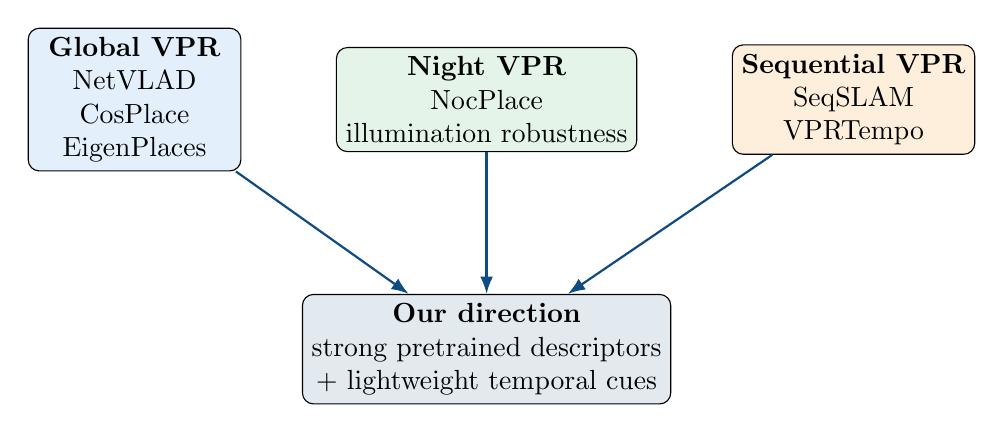
\begin{tikzpicture}[
    node distance=14mm and 12mm,
    box/.style={draw, rounded corners, minimum width=27mm, minimum height=11mm, align=center, fill=softgray},
    arrow/.style={-{Latex[length=2.2mm]}, thick, accent}
  ]
    \node[box, fill=softblue] (global) {\textbf{Global VPR}\\NetVLAD\\CosPlace\\EigenPlaces};
    \node[box, right=of global, fill=softgreen] (night) {\textbf{Night VPR}\\NocPlace\\illumination robustness};
    \node[box, right=of night, fill=softorange] (sequence) {\textbf{Sequential VPR}\\SeqSLAM\\VPRTempo};
    \node[box, below=18mm of night, minimum width=42mm, fill=accent!12] (ours) {\textbf{Our direction}\\strong pretrained descriptors\\+ lightweight temporal cues};
    \draw[arrow] (global) -- (ours);
    \draw[arrow] (night) -- (ours);
    \draw[arrow] (sequence) -- (ours);
  \end{tikzpicture}
  \end{center}

  \vspace{0.8em}
  \centering
  \pill{softblue}{Training-free bias} \hspace{1em}
  \pill{softgreen}{Benchmark + campus transfer} \hspace{1em}
  \pill{softorange}{Live demo focus}
\end{frame}

\begin{frame}{Data and Evaluation Setup}
  \begin{columns}[T,totalwidth=\textwidth]
    \column{0.46\textwidth}
      \begin{block}{Benchmark}
        \centering
        \Large GardensPoint

        \vspace{0.4em}
        \large controlled day-to-night evaluation
      \end{block}

      \vspace{0.5em}
      \begin{block}{Metrics}
        \centering
        \large AUC

        \vspace{0.2em}
        \large Recall@1 / 5 / 10

        \vspace{0.2em}
        \large Recall@100P
      \end{block}

    \column{0.50\textwidth}
      \begin{block}{Our campus dataset}
        \centering
        \large 50 day reference images

        \vspace{0.2em}
        \large 64 night queries

        \vspace{0.2em}
        \large 33 matched, 31 no-match
      \end{block}

      \vspace{0.6em}
      \centering
      
\includegraphics[width=0.44\linewidth,height=0.28\textheight,keepaspectratio]{../../custom_dataset/day_images/image001.jpg}
      \hfill
      
\includegraphics[width=0.44\linewidth,height=0.28\textheight,keepaspectratio]{../../custom_dataset/night_images/image001.jpg}
  \end{columns}
\end{frame}

\begin{frame}{Methodology}
  \begin{center}
  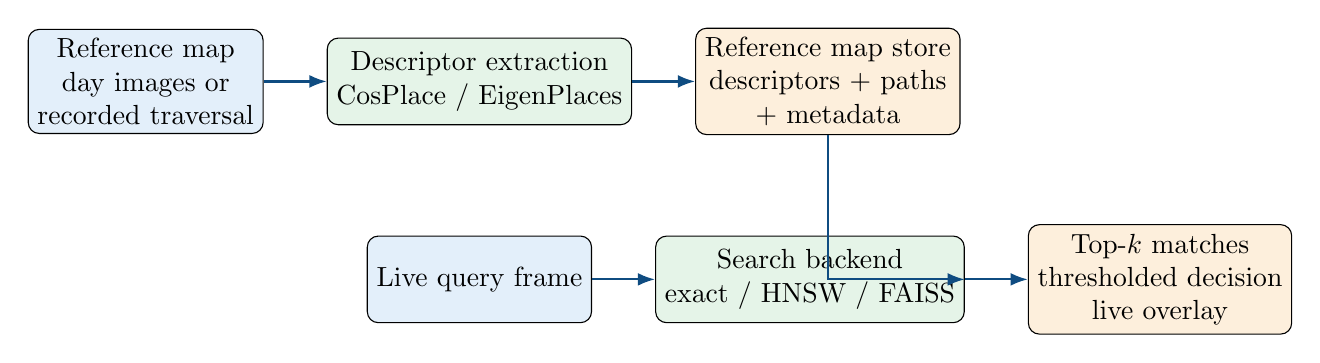
\begin{tikzpicture}[
    node distance=10mm and 8mm,
    box/.style={draw, rounded corners, minimum width=27mm, minimum height=11mm, align=center, fill=softgray},
    arrow/.style={-{Latex[length=2.2mm]}, thick, accent}
  ]
    \node[box, fill=softblue] (map) {Reference map\\day images or\\recorded traversal};
    \node[box, right=of map, fill=softgreen] (desc) {Descriptor extraction\\CosPlace / EigenPlaces};
    \node[box, right=of desc, fill=softorange] (store) {Reference map store\\descriptors + paths\\+ metadata};
    \node[box, below=14mm of desc, fill=softblue] (query) {Live query frame};
    \node[box, right=of query, fill=softgreen] (search) {Search backend\\exact / HNSW / FAISS};
    \node[box, right=of search, fill=softorange] (out) {Top-$k$ matches\\thresholded decision\\live overlay};

    \draw[arrow] (map) -- (desc);
    \draw[arrow] (desc) -- (store);
    \draw[arrow] (query) -- (search);
    \draw[arrow] (store) |- (search);
    \draw[arrow] (search) -- (out);
  \end{tikzpicture}
  \end{center}

  \vspace{0.8em}
  \begin{columns}[T,totalwidth=\textwidth]
    \column{0.33\textwidth}
      \centering \pill{softblue}{Offline: build map}
    \column{0.33\textwidth}
      \centering \pill{softgreen}{Online: search + rank}
    \column{0.33\textwidth}
      \centering \pill{softorange}{Demo: webcam / phone / robot}
  \end{columns}
\end{frame}

\begin{frame}{Live System Architecture}
  \begin{center}
  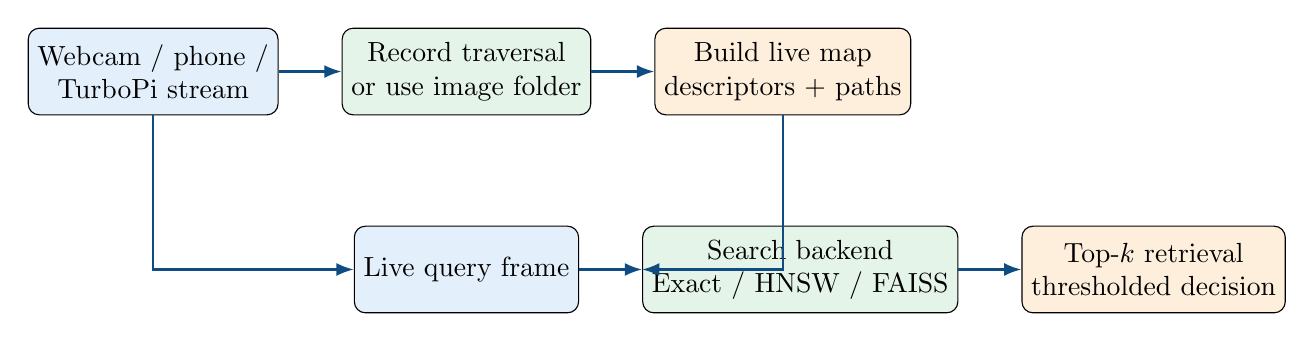
\begin{tikzpicture}[
    node distance=10mm and 8mm,
    box/.style={draw, rounded corners, minimum width=28mm, minimum height=11mm, align=center, fill=softgray},
    arrow/.style={-{Latex[length=2.2mm]}, thick, accent}
  ]
    \node[box, fill=softblue] (source) {Webcam / phone /\\TurboPi stream};
    \node[box, right=of source, fill=softgreen] (record) {Record traversal\\or use image folder};
    \node[box, right=of record, fill=softorange] (build) {Build live map\\descriptors + paths};
    \node[box, below=14mm of record, fill=softblue] (query) {Live query frame};
    \node[box, right=of query, fill=softgreen] (ann) {Search backend\\Exact / HNSW / FAISS};
    \node[box, right=of ann, fill=softorange] (decision) {Top-$k$ retrieval\\thresholded decision};

    \draw[arrow] (source) -- (record);
    \draw[arrow] (record) -- (build);
    \draw[arrow] (source) |- (query);
    \draw[arrow] (build) |- (ann);
    \draw[arrow] (query) -- (ann);
    \draw[arrow] (ann) -- (decision);
  \end{tikzpicture}
  \end{center}

  \vspace{0.9em}
  \begin{columns}[T,totalwidth=\textwidth]
    \column{0.32\textwidth}
      \centering \pill{softblue}{Config-driven pipeline}
    \column{0.32\textwidth}
      \centering \pill{softgreen}{Modular search layer}
    \column{0.32\textwidth}
      \centering \pill{softorange}{Ready for live demo}
  \end{columns}
\end{frame}

\begin{frame}{Benchmark Results}
  \begin{columns}[T,totalwidth=\textwidth]
    \column{0.58\textwidth}
      \centering
      \begin{tabular}{lcccc}
        \toprule
        \textbf{Model} & \textbf{AUC} & \textbf{R@1} & \textbf{R@5} & \textbf{R@10} \\
        \midrule
        CosPlace & 0.592 & 0.350 & 0.840 & 0.925 \\
        EigenPlaces & \textbf{0.676} & \textbf{0.370} & 0.840 & \textbf{0.940} \\
        AlexNet conv3 & 0.195 & 0.300 & 0.665 & 0.745 \\
        SAD & 0.030 & 0.090 & 0.225 & 0.305 \\
        \bottomrule
      \end{tabular}

      \vspace{0.8em}
      \centering
      \pill{softgreen}{Best baseline: EigenPlaces}

    \column{0.38\textwidth}
      \begin{block}{Takeaway}
        \centering
        \Large Top-5 is already strong

        \vspace{0.6em}
        \large Main gap: ranking the correct place first
      \end{block}
  \end{columns}
\end{frame}

\begin{frame}{Campus Transfer Results}
  \begin{columns}[T,totalwidth=\textwidth]
    \column{0.58\textwidth}
      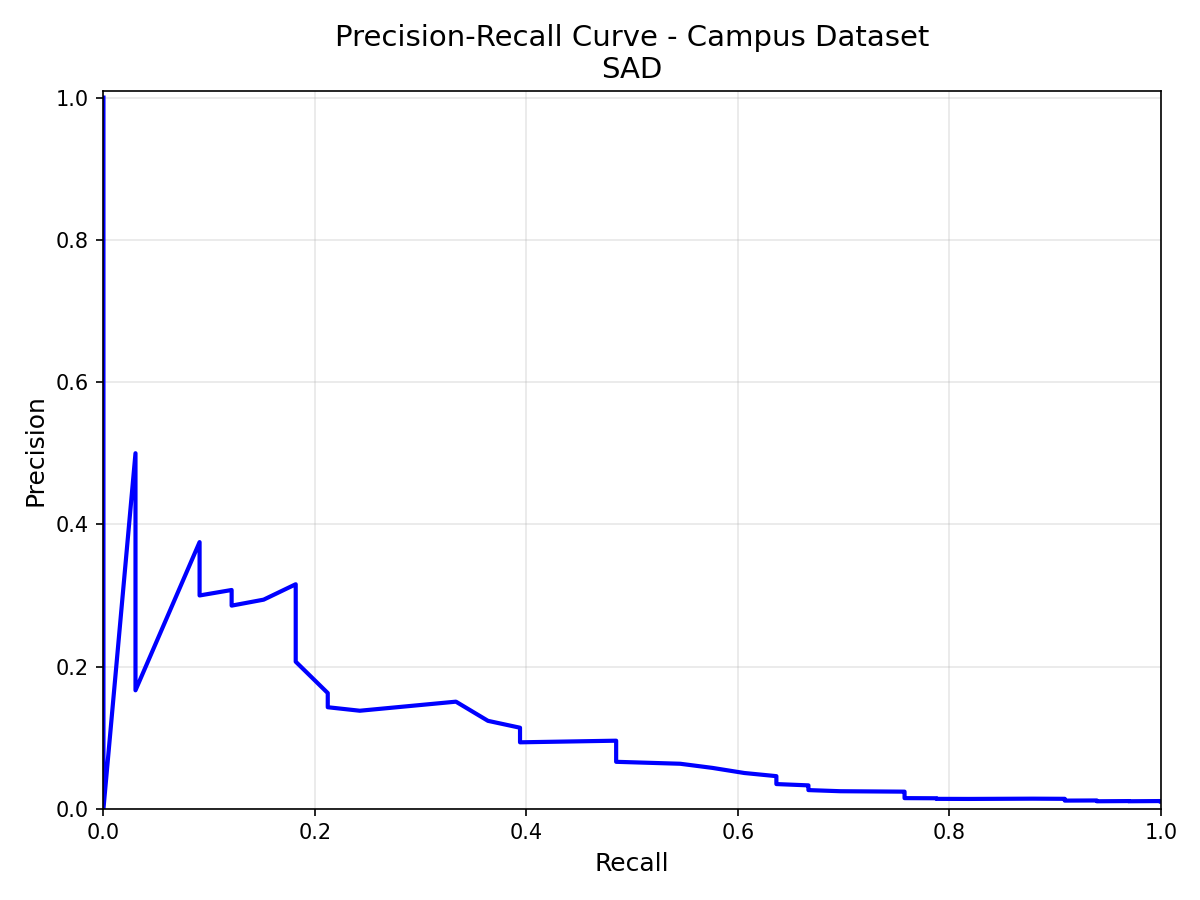
\includegraphics[width=\linewidth,height=0.72\textheight,keepaspectratio]{../../output_images/campus_pr_curve.png}

    \column{0.38\textwidth}
      \begin{block}{Campus / CosPlace}
        \centering
        \Large R@1 = 0.727

        \vspace{0.3em}
        \Large R@5 = 1.000

        \vspace{0.3em}
        \Large AUC = 0.470
      \end{block}

      \vspace{0.6em}
      \centering
      \pill{softblue}{50 day refs}

      \vspace{0.3em}
      \pill{softorange}{64 night queries}

      \vspace{0.3em}
      \pill{softgreen}{33 matched / 31 no-match}
  \end{columns}
\end{frame}

\begin{frame}{What We Learned From Relabeling}
  \begin{columns}[T,totalwidth=\textwidth]
    \column{0.52\textwidth}
      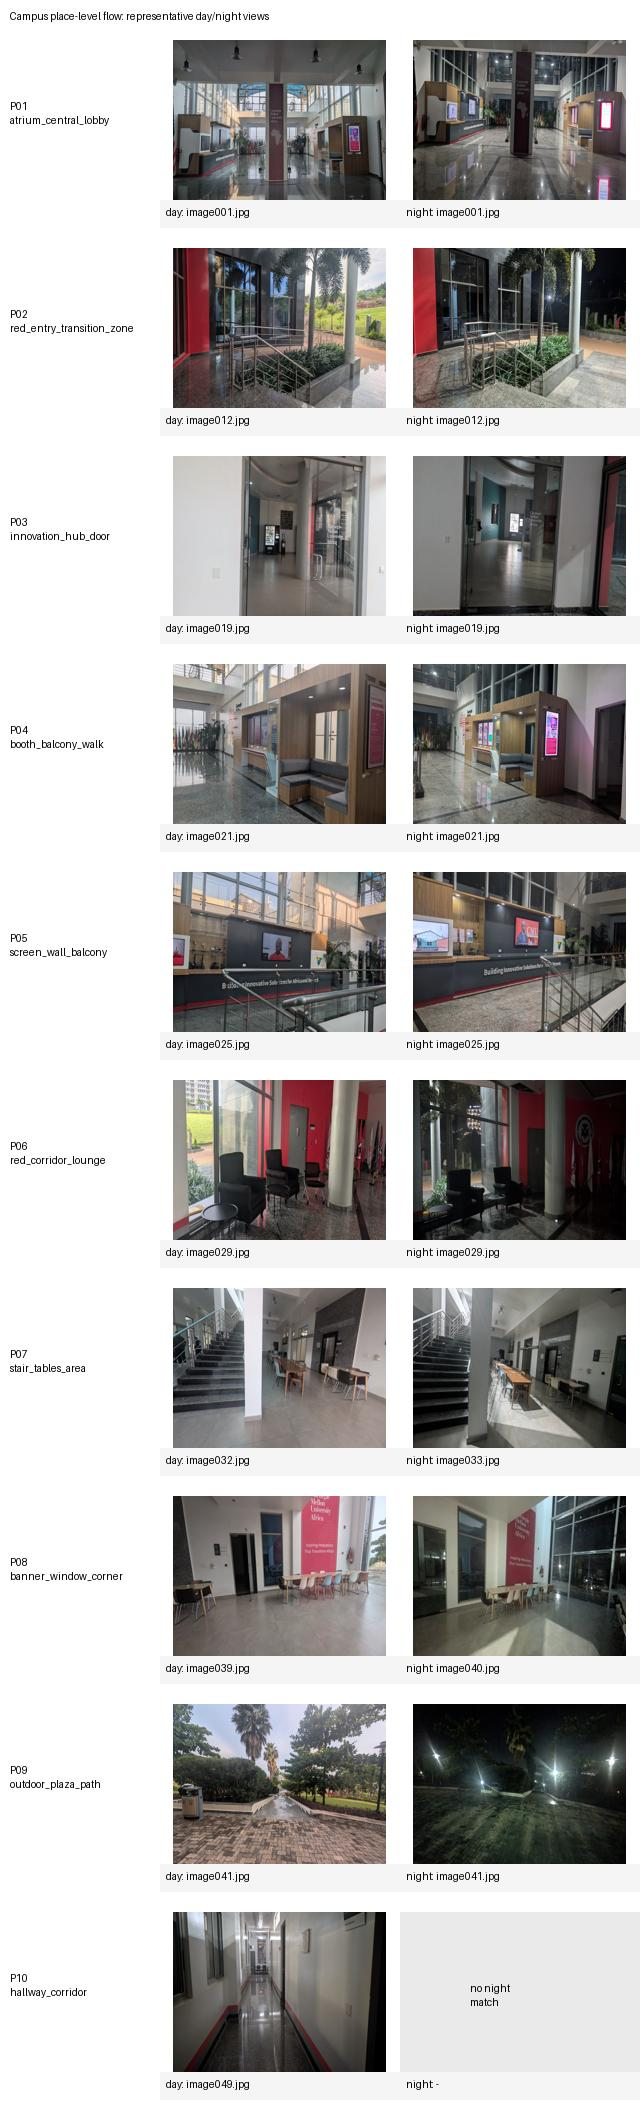
\includegraphics[width=\linewidth,height=0.63\textheight,keepaspectratio]{../../custom_dataset_place_level/place_flow_visual.jpg}

      \vspace{0.4em}
      \centering \pill{softgreen}{10 place IDs}

    \column{0.44\textwidth}
      \begin{block}{Main finding}
        \centering
        \Large Original campus setup

        \vspace{0.2em}
        \Large was too strict for

        \vspace{0.2em}
        \Large multi-view place recognition
      \end{block}

      \vspace{0.5em}
      \begin{block}{After place-level relabeling}
        \centering
        \large CosPlace: R@1 \ 0.727 $\rightarrow$ 0.969

        \vspace{0.2em}
        \large EigenPlaces: AUC \ 0.443 $\rightarrow$ 0.663

        \vspace{0.2em}
        \large NetVLAD: R@1 \ 0.394 $\rightarrow$ 0.891
      \end{block}
  \end{columns}
\end{frame}

\begin{frame}{Qualitative Result}
  \begin{columns}[T,totalwidth=\textwidth]
    \column{0.49\textwidth}
      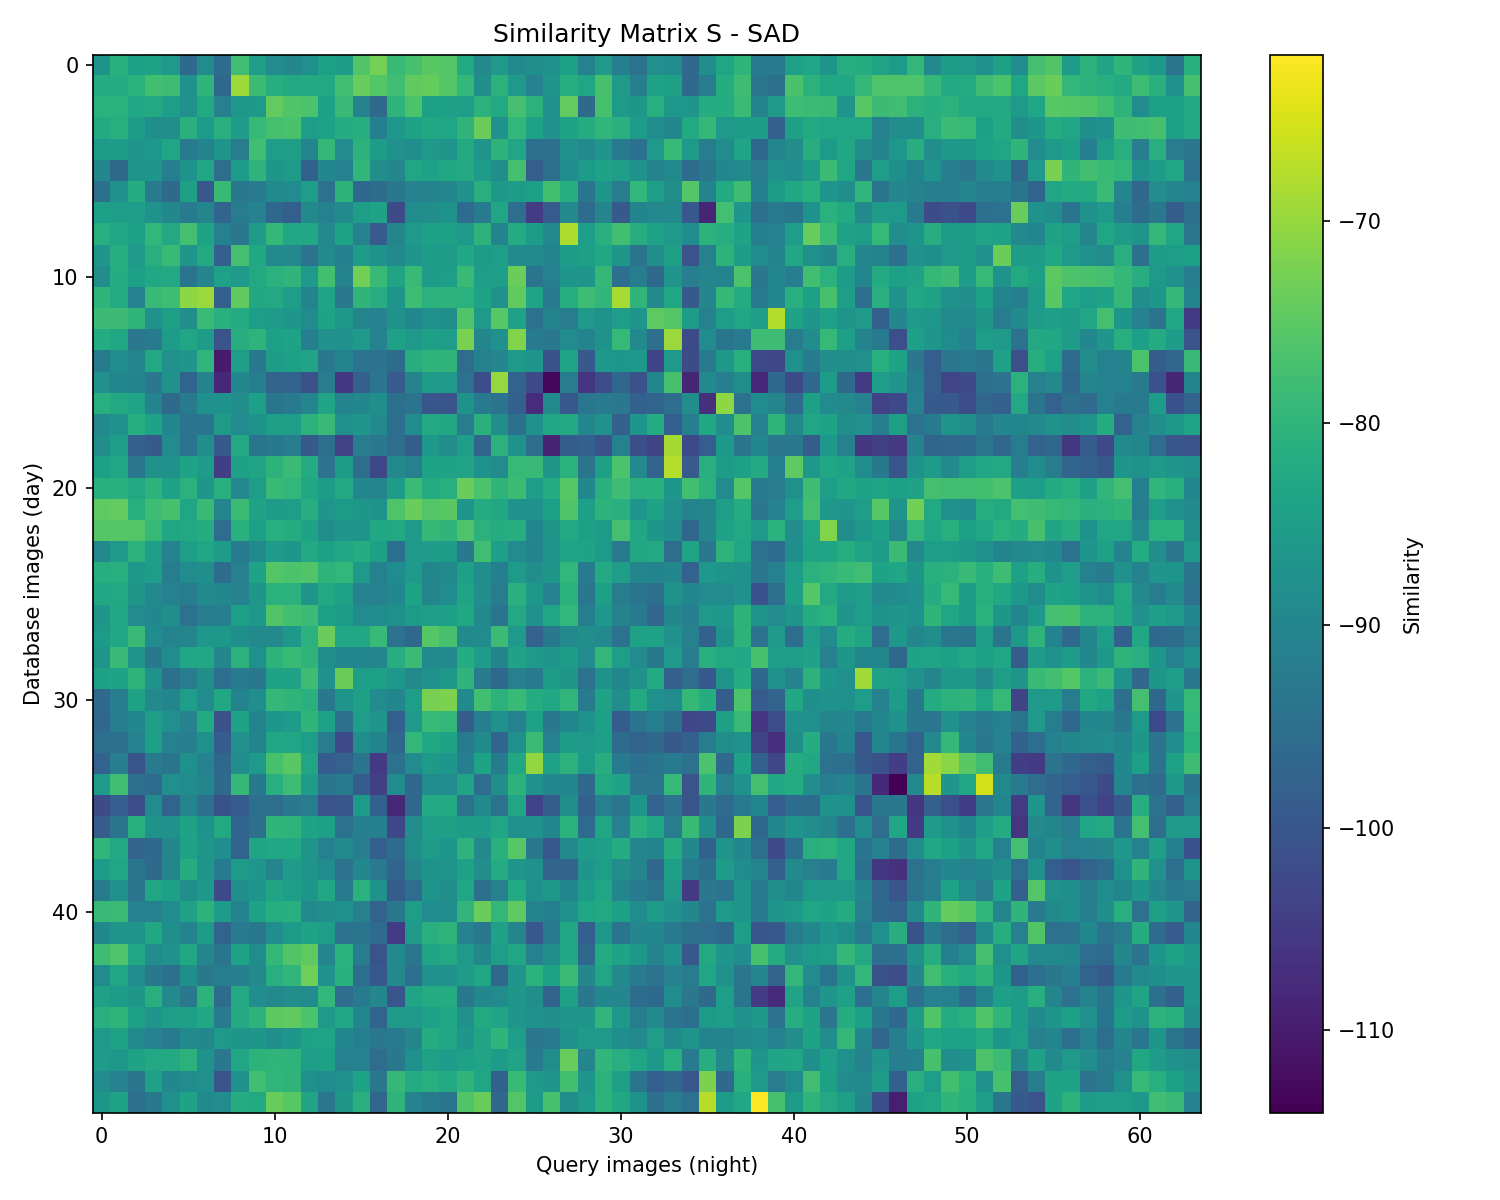
\includegraphics[width=\linewidth,height=0.68\textheight,keepaspectratio]{../../output_images/campus_similarity_matrix.png}

      \vspace{0.4em}
      \centering \pill{softblue}{Similarity structure}

    \column{0.49\textwidth}
      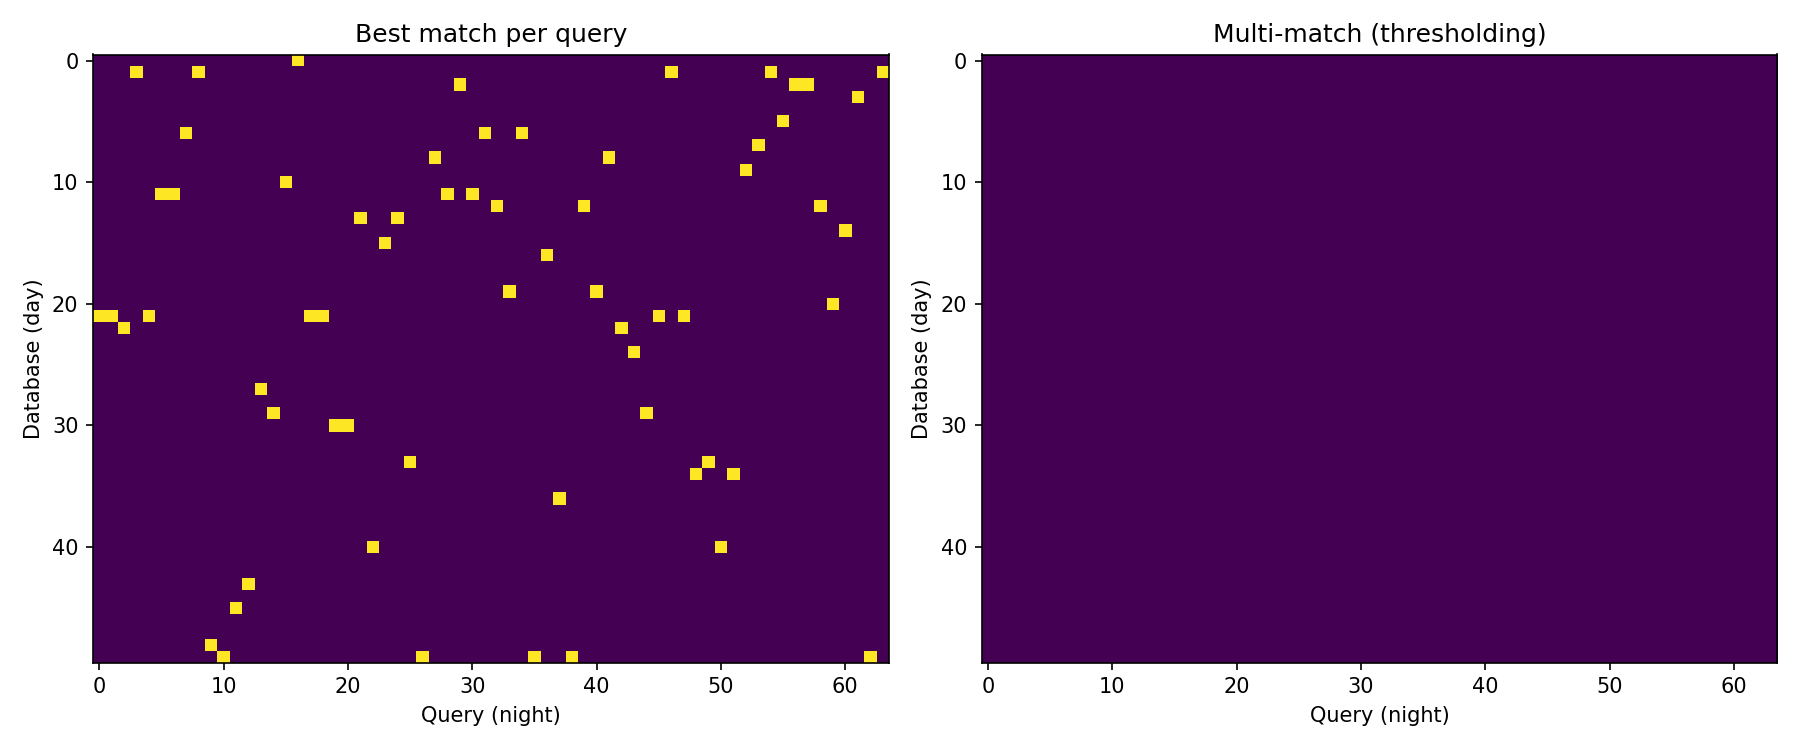
\includegraphics[width=\linewidth,height=0.68\textheight,keepaspectratio]{../../output_images/campus_matching_results.png}

      \vspace{0.4em}
      \centering \pill{softorange}{Correct vs wrong matches}
  \end{columns}
\end{frame}

\begin{frame}{What We Built Beyond Offline Evaluation}
  \begin{columns}[T,totalwidth=\textwidth]
    \column{0.48\textwidth}
      
\includegraphics[width=\linewidth,height=0.34\textheight,keepaspectratio]{../../custom_dataset/day_images/image010.jpg}

      \vspace{0.6em}
      
\includegraphics[width=\linewidth,height=0.34\textheight,keepaspectratio]{../../custom_dataset/night_images/image010.jpg}

    \column{0.48\textwidth}
      \begin{block}{Current practical pipeline}
        \centering
        \large Build map from images or traversal video

        \vspace{0.4em}
        \large Run live localization from webcam / stream

        \vspace{0.4em}
        \large Swap search backends through config
      \end{block}

      \vspace{0.6em}
      \centering
      \pill{softblue}{Applied CV emphasis}

      \vspace{0.3em}
      \pill{softgreen}{Robot-facing deployment}

      \vspace{0.3em}
      \pill{softorange}{Demo-ready workflow}
  \end{columns}
\end{frame}

\begin{frame}{Conclusion}
  \begin{columns}[T,totalwidth=\textwidth]
    \column{0.32\textwidth}
      \begin{block}{1}
        \centering
        \Large Strong benchmark baseline
      \end{block}

    \column{0.32\textwidth}
      \begin{block}{2}
        \centering
        \Large Campus transfer improved after place-level relabeling
      \end{block}

    \column{0.32\textwidth}
      \begin{block}{3}
        \centering
        \Large End-to-end live system is in place
      \end{block}
  \end{columns}

  \vspace{1em}
  \centering
  \pill{softblue}{Key takeaway: strict labels under-credited multi-view matches} \hspace{0.8em}
  \pill{softgreen}{Search at larger map scale} \hspace{0.8em}
  \pill{softorange}{Robust live demo}
\end{frame}

\begin{frame}{Presentation Logistics and Deliverables}
  \begin{columns}[T,totalwidth=\textwidth]
    \column{0.48\textwidth}
      \begin{block}{Presentation}
        \centering
        \Large Apr 26, 2026

        \vspace{0.3em}
        \Large 2:00 PM, F203

        \vspace{0.6em}
        \large 8 min talk + 4 min Q\&A

        \vspace{0.4em}
        \large Random presentation order
      \end{block}

    \column{0.48\textwidth}
      \begin{block}{Submission}
        \centering
        \large 5-min video presentation

        \vspace{0.3em}
        \large Due Apr 25, 11:59 PM

        \vspace{0.6em}
        \large Final report + reproducible GitHub + demo link

        \vspace{0.3em}
        \large Due Apr 30, 11:59 PM CAT
      \end{block}
  \end{columns}
\end{frame}

\begin{frame}[plain]
  \centering
  \vspace{2.2cm}
  {\Huge \textbf{Thank you}}

  \vspace{1.2em}
  {\Large Demo / Questions}
\end{frame}

\end{document}
